\chapter{Generalised Kibble-Zurek scaling in a spin-1 BEC}\label{chap: spin-1}


\section{Introduction}
Nonequilibrium phase transitions arise in many areas of physics, ranging from
cosmology to condensed matter~\cite{Polkovnikov2011}.
Unlike its classical counterpart, a quantum phase transition (QPT) is a
zero-temperature transition driven by quantum fluctuations~\cite{Sachdev2011}.
In such a transition, a fundamental change of ground state occurs as an external
parameter is varied across the quantum critical point.
As this critical point is passed, the timescale governing the dynamics diverges,
resulting in the system no longer adiabatically following the ground state.
This non-adiabatic evolution breaks the symmetry of the system, which typically
results in the formation of topological defects.
The Kibble-Zurek mechanism (KZM) is a theory that describes the resulting
dynamics and predicts the scaling properties of the excitations from the details
of the universality class of the transition.
It was first introduced by Kibble in the context of the topology of cosmic
strings in the early universe~\cite{Kibble1976, Kibble1980}, before being
extended by Zurek to condensed matter systems~\cite{Zurek1985, Zurek1993,
    Zurek1996}.


The standard KZ theory is very general, and can be applied to any continuous
phase transition.
The robustness of the theory has seen it successfully applied to both
classical~\cite{Donadello2016,Beugnon2017} and
quantum~\cite{Dziarmaga2005, Damski2005, Lamacraft2007} phase transitions.
Whilst the theory has had great success in applications to continuous,
second-order transitions, direct application to discontinuous transitions
does not give an accurate description of observed scaling laws.
Recently, there has been the first experimental evidence of the existence of
scaling laws for a first-order QPT~\cite{Qiu2020}, where standard KZ theory
failed to predict the observed scaling.
However, the KZM was generalised by considering the energy gap between the
metastable state and its first corresponding excited state, which then gave an
accurate prediction of the observed scaling laws.
There is current interest in trying to generalise the KZM and applying it to
discontinuous transitions and deriving appropriate scaling
laws~\cite{Divakaran2008, Suzuki2015}.

Fisher and Berker, in the classical case, first discussed a particular type of
discontinuous, first-order transition and introduced the notion of a
discontinuous critical point (DCP)~\cite{Fisher1982}.
The DCP separates two distinct phases, characterized by a discontinuous jump
in the order parameter.
Despite the discontinuity, the transition can still be characterized by a
diverging length scale and hence critical exponents can be derived.
This framework was then extended to the quantum case, specifying the conditions
for a quantum discontinuous critical point (QDCP)~\cite{Suzuki2015}.
The QDCP leads to a prediction of the scaling of the defect density that is
modified from the typical KZ scenario.

Spinor Bose-Einstein condensates (BECs) offer a highly controllable platform
for studying non-equilibrium physics, ranging from topological
defects~\cite{Lovegrove2014, Borgh2016} to quantum
quenches~\cite{Symes2017, Prufer2018, Schmied2019}.
\textcolor{red}{More references/topics?}
In addition, their rich phase diagram has seen the KZM applied both numerically
and experimentally in various continuous phase transitions~\cite{Damski2007,
    Saito2007, Saito2007a, Swislocki2013, Witkowska2013, Anquez2016}.
For a ferromagnetic spin-1 BEC, there exists a first-order QPT between a
three-component broken-axisymmetry (BA) phase and a ferromagnetic (FM) phase,
making this system an ideal platform for investigating the KZM across
discontinuous transitions.

\section{The Kibble-Zurek mechanism}\label{sec: the-KZM}
Consider a system that undergoes a spontaneous breaking of symmetry when a
control parameter, \( \lambda \), is ramped across a phase transition that
occurs at the critical point, \( \lambda_c \).
A continuous, second-order phase transition can be characterized by a divergence
of the equilibrium correlation length
\begin{equation}
    \xi(\epsilon) \sim |\epsilon|^{-\nu},
\end{equation}
and an equilibrium relaxation time
\begin{equation}
    \tau(\epsilon) \sim \xi^z \sim |\epsilon|^{-\nu z},
    \label{eq: equil-relax-time}
\end{equation}
where
\begin{equation}
    \epsilon = \frac{\lambda - \lambda_c}{\lambda_c}
\end{equation}
is the dimensionless distance from the critical point.
The equilibrium relaxation time \( \tau \) describes the time it takes for the
system to react to an external change of a parameter.
In a quantum phase transition, the relaxation time is set by the inverse of an
energy gap \( \Delta \) between the ground state and the first excited
state~\cite{Zurek2005, Damski2006}
\begin{equation}
    \tau \simeq \Delta^{-1}.
\end{equation}
As we approach the critical point, the energy gap vanishes as
\begin{equation}
    \Delta \sim |\epsilon|^{\nu z}.
\end{equation}

The system is initially prepared in a high-symmetry phase (\(  \epsilon > 0 \)),
but breaks that symmetry as the critical point is crossed (\(  \epsilon < 0 \)).
In the above equations, the exponents \(  z \) and \( \nu \) are the dynamical
and correlation length critical exponents, respectively.
These exponents are determined by the universality class of the phase
transition~\cite{Sachdev2011}, and different systems belonging to the same
universality class share the same critical exponents.

The KZM describes the dynamics of crossing the critical point when \( \lambda \)
is continually varied.
We assume the form of a linear quench (cases concerning non-linear quenches are
discussed in Refs.~\cite{Barankov2008,Mondal2009}), such that the control
parameter can be written as
\begin{equation}
    \lambda(t) = \lambda_c - \epsilon(t),
\end{equation}
where the distance to the critical point is
\begin{equation}
    \epsilon(t) = \frac{t}{\tau_Q}
    \label{eq: time-dependent-epsilon}
\end{equation}
for a quench time \( \tau_Q \).
This form gives a transition rate \( |\dot{\epsilon}/{\epsilon}|=t^{-1} \) which
diverges as we approach the critical point.
Here, \( t \in [-\tau_Q, \tau_Q] \), where the critical point is reached at
\( t=0 \).
The dynamics of the system can be broken into three stages as \( \epsilon \) is
ramped from \( \epsilon > 0 \) to \( \epsilon < 0 \): adiabatic, frozen, and
adiabatic again (see Fig.~\ref{fig: adiabatic-impulse} for a schematic
representation).
\begin{figure}
    \centering
    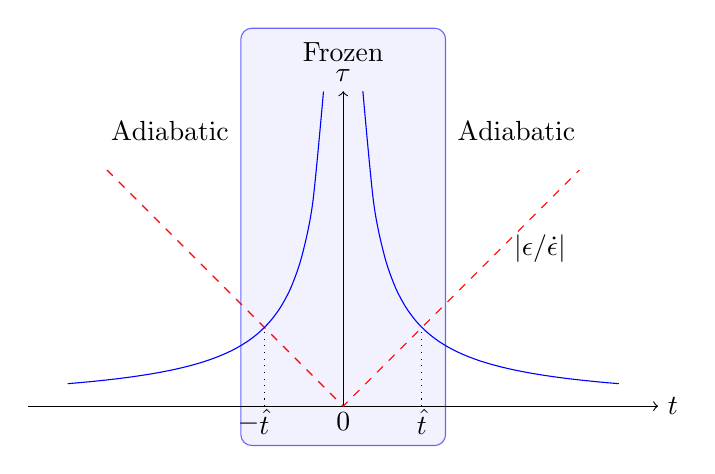
\begin{tikzpicture}
        \filldraw[color=blue!60, fill=blue!5, rounded corners] (-1.3, -0.5)
        rectangle (1.3, 4.8);
        \draw[->] (-4, 0) -- (4, 0) node[right] {\( t \)};
        \draw[->] (0, 0) -- (0, 4) node[above] {$\tau$};
        \draw[scale=1, domain=-3:3, dashed, variable=\x, red] plot
        ({\x}, {abs(\x)});
        \draw[scale=1, domain=0.25:3.5, smooth, variable=\x, blue] plot
        ({\x}, {\x^(-1)});
        \draw[scale=1, domain=-3.5:-0.25, smooth, variable=\x, blue] plot
        ({\x}, {abs(\x^(-1))});
        \node at (1, -0.2) {\( \hat{t} \)};
        \node at (-1, -0.2) {\( \hat{t} \)};
        \node at (-1.2, -0.22) {$-$};
        \draw[dotted] (1, 0) -- (1, 1);
        \draw[dotted] (-1, 0) -- (-1, 1);
        \node at (0, 4.5) {Frozen};
        \node at (2.5, 2) {$|\epsilon/\dot{\epsilon}|$};
        \node at (2.2, 3.5) {Adiabatic};
        \node at (-2.2, 3.5) {Adiabatic};
        \node at (0, -0.2) {$0$};
    \end{tikzpicture}
    \caption[Schematic representation of the dynamics of a system during a
        linear quench]
    {A schematic representation of the dynamics of a system during a
        linear quench. The system starts in a high-symmetry phase (\( t > 0 \)) and
        is quenched across a critical point to a low symmetry phase (\( t < 0 \)) by
        the reduced control parameter (red dashed line) \( \epsilon(t) = t/\tau_q \).
        As the critical point is approached, the equilibrium relaxation time
        (blue line) diverges, and the order parameter can no longer follow the
        ground state, leading to frozen dynamics in the interval
        \( t \in [-\hat{t}, \hat{t}] \)}.\label{fig: adiabatic-impulse}
\end{figure}

Far from the critical point, the equilibrium relaxation time is small compared
to the inverse transition rate \( |\epsilon/\dot{\epsilon}| \), meaning the system
adiabatically follows the instantaneous ground state for \( \epsilon(t) \).
This stage of adiabaticity lasts until the instant
\begin{equation}
    \tau \approx |\epsilon/\dot{\epsilon}|=t.
    \label{eq: freeze-out-equal}
\end{equation}
Solving this equation yields the freeze-out time, \( \hat{t} \):
\begin{equation}
    \hat{t} \sim \tau_Q^\frac{z\nu}{1 + z\nu}.
    \label{eq: freeze-out-scaling}
\end{equation}
After this point is passed, however, the relaxation time diverges and the system
can no longer keep up with the externally imposed changes.
The system then enters the so-called impulse regime, where the dynamics are
frozen and remains in this regime until \( -\hat{t} \), when the relaxation
time becomes faster than the transition rate once again.
The consequence of the impulse region, however, is that the system arrives at
\( -\hat{t} \), which is in a broken-symmetry phase, whilst remaining
in the state set at \( \hat{t} \), which is in a symmetric phase.
This state at \( \hat{t} \) then becomes the initial state for the last adiabatic
stage of evolution beginning at \( -\hat{t} \).
At this point, the system is no longer in its current ground state and rectifies
this by breaking the symmetry of the initial state.
This results in the formation of distinct domains in the system whose size is
set by the value of the equilibrium correlation length at the freeze-out time
\begin{equation}
    \hat{\xi}=\xi(\hat{t}) \sim \tau_Q^{\frac{\nu}{1 + z\nu}}.
    \label{eq: KZM-domain-size}
\end{equation}
If the system supports topological defects such as vortices, then the defect
density is given by
\begin{equation}
    n_d \simeq \hat{\xi}^{-d} \sim \tau_Q^{\frac{-d\nu}{1+z\nu}},
\end{equation}
where \( d \) is the number of spatial dimensions.
This is a key result of the Kibble-Zurek mechanism and provides a
foundation in testing the KZM in BEC systems~\cite{Damski2007, Swislocki2013,
    Anquez2016, Saito2007, Saito2007a}.

\section{Numerical studies of the KZM across a second-order phase transition}
As shown in Sec.~\ref{sec: ground-states-spin-1}, there are four ground states
phases of spin-1 Bose-Einstein condensates; namely, the ferromagnetic,
antiferromagnetic, polar, and broken-axisymmetry phases, where each ground
state phase has an associated symmetry.
The Kibble-Zurek mechanism can be studied in spin-1 BECs by considering how
the change of a control parameter causes the order parameter to change from
one ground state to another.
As it does this, the symmetry of the system is spontaneously broken, and hence
the Kibble-Zurek theory can be applied.

Spin-1 BECs support numerous first- and second-order phase transitions
when the linear, \( p \), or quadratic, \( q \), Zeeman shifts are
ramped across a critical point~\cite{Kawaguchi2012}.
A second-order transition is characterised by the derivative of the energy with
respect to \( p \) and \( q \) change continuously across the transition
\textcolor{red}{? (Are there other conditions on a second-order transition?)}.
In this section, we aim to test the predictions of the Kibble-Zurek mechanism
for a second-order phase transition in a spin-1 BEC\@.

\subsection{Polar to broken-axisymmetry quench}\label{sec: KZM-second-order-numerics}
Motivated by previous work~\cite{Damski2007}, we will investigate the
Kibble-Zurek mechanism across the second-order phase transition occurring
between the polar and broken-axisymmetry phases in a ferromagnetic spin-1 BEC\@.
The polar phase is the energetic ground state when \( Q=q/|c_1|n > 2 \).
The critical point \( Q = 2 \) represents the second-order phase transition to
the BA phase.
The BA phase contains three Bogoliubov modes~\cite{Uchino2010}, but only one
is non-zero in the long wavelength limit (see
Sec.~\ref{subsec: bogoliubov-modes} for further details on Bogoliubov modes in
a spin-1 BEC).
This mode is gapped, and has the scaling form
\begin{equation}
    \Delta \sim \sqrt{4 - q^2}.
\end{equation}
\textcolor{red}{We need to figure out why they take the scaling from the BA side
    and not the polar side.}

We assume the form of a linear quench
\begin{equation}
    Q(t) = 2 - \frac{t}{\tau_Q},
    \label{eq: time-dep-Q-damski}
\end{equation}
where \( \tau_Q \) is the quench time.
To investigate Kibble-Zurek scaling, we consider the freeze-out time,
\( \hat{t} \), which occurs when the equilibrium relaxation time is equal to the
rate of change of the control parameter [see Eq.~\eqref{eq: freeze-out-equal}].
Using the above equation and considering sufficiently slow quenches
(\(\tau_Q \gg 1\)), this leads to
\begin{equation}
    \hat{t} \sim \tau_Q^{\frac{1}{3}}.
\end{equation}
\textcolor{red}{I've tried deriving this and I am getting stuck\ldots}

We now analyse the resulting dynamics when linearly decreasing \( q \) according
to Eq.~\eqref{eq: time-dep-Q-damski}.
We start from the polar phase (\( t < 0 \)) and end the simulation precisely at
\( Q = 0 \) (\( t=2\tau_Q \)) in the BA phase.
The initial state is a polar wave function that is slightly perturbed:
\begin{equation}
    \psi = \left(\delta\psi_1, \frac{1}{\sqrt{L}} + \delta\psi_0,
    \delta\psi_{-1}\right),
    \label{eq: peturbed-polar-initi-state}
\end{equation}
where \( |\delta\psi_m| \ll 1 / \sqrt{L} \) are small noise terms and \( L \) is
the length.
The real and imaginary parts of these terms at individual grid points are drawn
from the probability distribution
\( p(x) = \exp(-x^2/2\sigma^2)/\sqrt{2\pi}\sigma \).
To ensure we remain close to the polar ground state, we take
\( \sigma=10^{-4} \).

We consider a 1D system with \(N_x = 2048\) grid points with \(L=78\) and
choose dimensionless spin-independent interaction \(c_0=1.4\times10^5\) and
\(c_0/c_1 = -222\).
We start with the initial state in Eq.~\eqref{eq: peturbed-polar-initi-state}
and integrate the spin-1 Gross-Pitaevskii equations~\cite{Symes2016}.

\subsection{Evolution of the transverse magnetisation}
To determine the freeze-out time within our system, we need to find a quantity
that grows as the transition point is crossed.
This freeze-out time is then measured by the time it takes for the onset of
that growth to occur.
The quantity that satisfies this condition in the polar to BA transition is the
transverse magnetisation
\begin{equation}
    M_\perp = \int f_x^2 + f_y^2 \, dz,
\end{equation}
where \(f_x\) and \(f_y \) are the \(x, y\) components of the condensate spin
vector, respectively.
In the polar phase this quantity is zero, but becomes non-zero in the BA limit
where it is \(M_\perp = (1 - Q^2/4)/L\).
\begin{figure}
    \centering
    \begin{subfigure}{0.49\textwidth}
        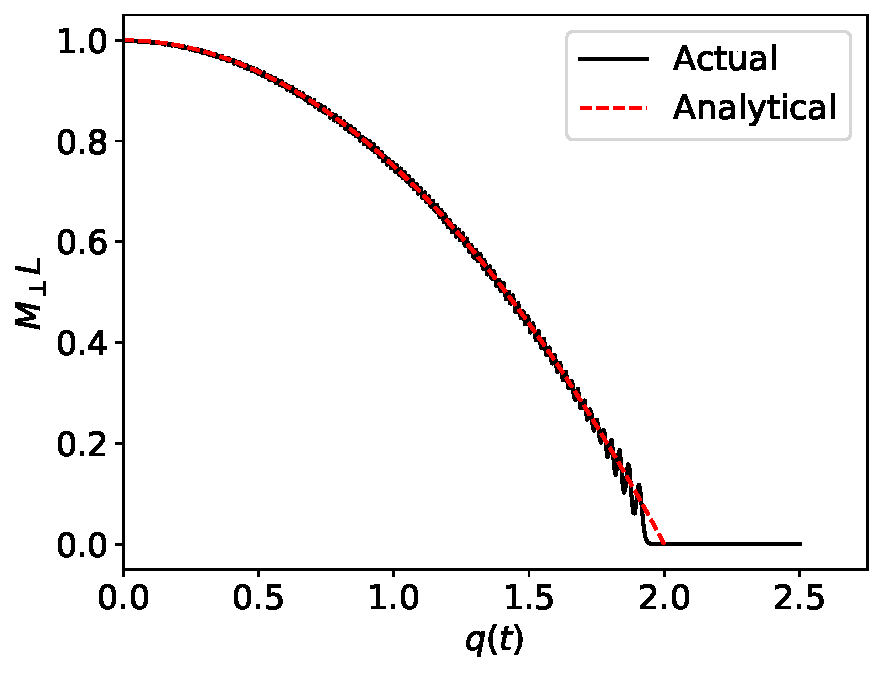
\includegraphics[width=\textwidth]{gfx/ch-spin1/magnetisation_vs_Q.pdf}
        \caption{\label{subfig: magnetisation-vs-Q}}
    \end{subfigure}
    \begin{subfigure}{0.49\textwidth}
        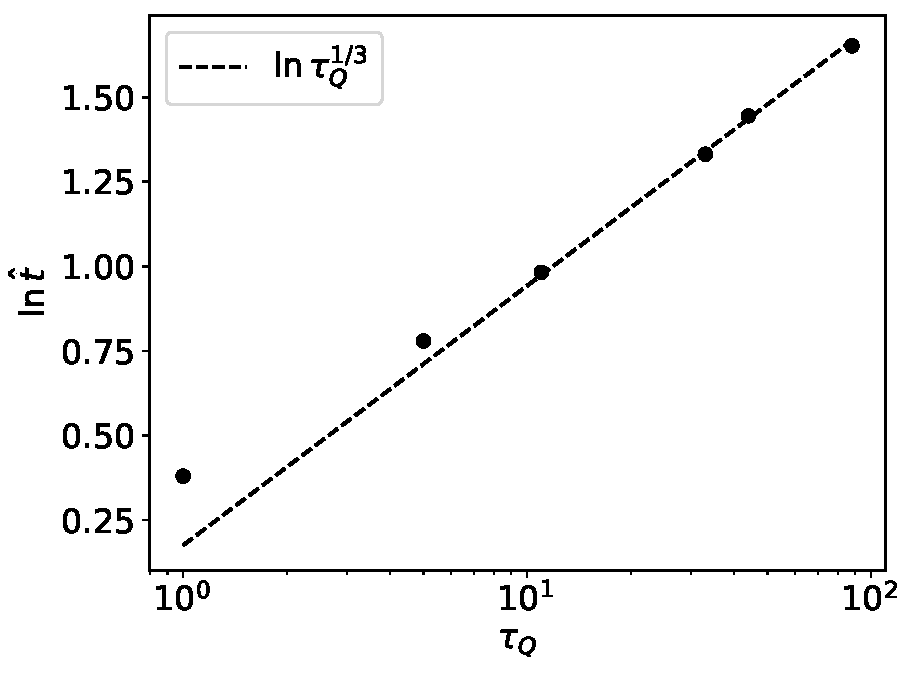
\includegraphics[width=\textwidth]{gfx/ch-spin1/t-hat_vs_tau_q.pdf}
        \caption{\label{subfig: t-hat-vs-tau-q}}
    \end{subfigure}
    \caption[Transverse magnetisation for as a function of quench parameter,
        \(Q\)]
    {(a) The transverse magnetisation as a function of \( Q(t) \) for
        \(\tau_Q=11\).
        Plotted are the numerical values (black line) and the
        analytical prediction (red line).
        (b) The extracted value of \( \hat{t} \) versus the quench time.
        Overlaid is the power-law scaling \(\tau_Q^{1/3}\).}
\end{figure}
Fig.~\ref{subfig: magnetisation-vs-Q} shows a typical evolution of the
transverse magnetisation for \(\tau_Q = 11\).
One sees that after the critical point is crossed at \( Q = 2 \), the transverse
magnetisation grows in a non-trivial fashion.
This growth starts precisely after the system exits the freeze-out stage, which
occurs at \(t=\hat{t}\).
The magnetisation then grows rapidly, exceeding the analytical prediction in
places, and begins to oscillate with the amplitude decaying over time.
Using this quantity, we can test the Kibble-Zurek prediction in
Eq.~\eqref{eq: freeze-out-scaling}.

We define \( \hat{t} \) as the instant \(M_\perp L\) intersects 1\% of its
maximum value \(M_\perp L = 1\).
Fig~\ref{subfig: t-hat-vs-tau-q} shows the extracted value of \( \hat{t} \) for
a range of \( \tau_Q \).
We see an unambiguous power-law scaling of \(\tau_Q^{1/3}\) for
\(\tau_Q \geq 10\).
The gradual departure from the \(\hat{t} \sim \tau_Q^{1/3}\) scaling indicates
that the quench has to be sufficiently slow to capture the Kibble-Zurek scaling.
We note that the choice of 1\% here is arbitrary.
We tested a range of values up to a maximum of 10\%, and obtain quantitatively
similar behaviour for all values tested.

\section{Extending the KZ theory to first-order phase transitions}
The preceding sections were concerned with the KZM across second-order phase
transitions.
Describing the KZM across discontinuous, first-order transitions, however, has
been difficult due to lack of
universality~\cite{Turban2002,Continentino2004,Nauenberg1975a}.
More recent work has aimed to bridge the gap between the KZM and first-order
transitions~\cite{Suzuki2015}, and here we present an overview of how the KZM
can be adapted to fit a discontinuous phase transition.

Fisher and Berker~\cite{Fisher1982} presented the universality class for
a first-order phase transition known as a discontinuous critical point (DCP).
This DCP results in a discontinuity in the order parameter as the critical point
is passed.
Despite this, the transition can still be characterised by a diverging length
scale, and hence, critical exponents can be derived.
Suzuki \textit{et al.}~\cite{Suzuki2015} aimed to extend the notion of a DCP to
the quantum case and established the quantum discontinuous critical point
(QDCP).

Let us consider a system that contains a critical point at
\( q = q_c \), where \( q \) is a tunable parameter and contains
the presence of a symmetry-breaking field, \( p \).
For one to have a QDCP five conditions need to be satisfied~\cite{Suzuki2015}.
Firstly, the energy density \( \epsilon(q, p) \) must be a continuous
function of \( q \) and \( p \) across the critical point
\begin{equation}
    \epsilon(q_c + 0, 0) = \epsilon(q_c - 0, 0).
    \label{eq: continuous-energy-cond}
\end{equation}
The derivative of this energy density, however, is discontinuous
\begin{equation}
    \pdv{\epsilon(q_c + 0, 0)}{t} \neq \pdv{\epsilon(q_c - 0, 0)}{t}.
\end{equation}
The order parameter \( m(q, p) \), where
\( m=-\pdv{\epsilon(q, p)}{p} \)
\textcolor{red}{where does this come from?},
has a discontinuous jump as a function of \( q \) as the critical point is
passed
\begin{equation}
    |m(q_c - 0, 0)| > m(q_c + 0, 0)| = 0,
\end{equation}
whilst also having a discontinuous jump as a function of \( p \)
\begin{equation}
    |m(q_c, \pm 0)| > 0.
\end{equation}
Finally, we require that the derivative of the energy density be bounded as
\( q \rightarrow q_c \pm 0 \)
\begin{equation}
    \left|\pdv{\epsilon(q_c \pm 0, 0)}{q}\right| < \infty.
    \label{eq: bounded-energy-derivative-cond}
\end{equation}
These five conditions encapsulate a QDCP\@.

\subsection{BA to FM transition as a QDCP}
Let us now consider a specific example.
We are interested in the phase transition that occurs between the
broken-axisymmetry (BA) and ferromagnetic (FM) phases.
The energy densities for the two states are given by~\cite{Kawaguchi2012}
\begin{equation}
    \epsilon_\mathrm{BA} = \frac{{(-p^2 + q^2 +2qc_1n)}^2}{8c_1nq^2}
    + \frac{1}{2}c_0n, \qquad
    \epsilon_\mathrm{FM_{\pm}} = \mp p + q + \frac{1}{2}n(c_0 + c_1),
\end{equation}
where \( \epsilon_\mathrm{FM_{\pm}} \) corresponds to the energy density in the
FM phase for the spinor \( \zeta = {(1, 0, 0)}^T \) (+) and
\( \zeta = {(0, 0, 1)}^T \) (-).
One sees that at the critical point \( q=q_c=0 \) and \( p=0 \) the energy is
continuous.
The derivative of the above energies with respect to \( q \) yields
\begin{equation}
    \pdv{\epsilon_\mathrm{BA}}{q} =
    \frac{1}{4c_1n}\left(q - \frac{p^4}{q^3}\right) - \frac{p^2}{q^2}
    + \frac{1}{2},
    \qquad
    \pdv{\epsilon_\mathrm{FM_{\pm}}}{q} = 1.
\end{equation}
Indeed, there is a discontinuity in these derivatives at \( q=p=0 \), however,
they still remain bounded.
The relevant order parameter for this transition are given by
\begin{equation}
    m_\mathrm{BA} = \frac{p(p^2 - q^2 - 2qc_1n)}{8c_1nq},
    \qquad
    m_{\mathrm{FM}_{\pm}} = \pm 1,
\end{equation}
which is precisely the local magnetisation, \(F_z = |\psi_1|^2
- |\psi_{-1}|^2\), in both phases (see Sec.~\ref{sec: ground-states-spin-1}).
Again, one sees that at the critical point and for \( p=0 \) the order parameter
becomes zero in the BA phase whilst becoming non-zero in the FM phase.
In addition, as the linear Zeeman shift \( p \) is varied both above and below
zero the order parameter becomes non-zero.
We have shown that the BA to FM phase transition satisfies all conditions
specified in Eqs.~\eqref{eq: continuous-energy-cond}
-\eqref{eq: bounded-energy-derivative-cond}
and therefore is a QDCP\@.

\subsection{Predicting the density of defects}
Recall from Sec~\ref{sec: the-KZM} that the density of defects takes the form
\(N_d \simeq \xi^{-d}\).
Therefore, to predict the density of defects for the BA to FM transition, we
need to find the appropriate form for the correlation length, \(\xi \).
To do so, we consider the Bogoliubov modes of a spin-1 BEC\@.

Here, we derive each mode  of the BA phase explicitly from the relevant
Bogoliubov transformations and determine the relevant mode for the 
BA to FM transition.
The broken-axisymmetry phase of a spin-1 BEC exhibits three Bogoliubov
modes~\cite{Uchino2010}.
The broken-axisymmetry phase can be parameterised as
\begin{align}
    \zeta^\text{BA} = \left(\frac{\sin\theta}{\sqrt{2}}, \cos\theta,
    \frac{\sin\theta}{\sqrt{2}}\right),
\end{align}
where \(\sin\theta = \sqrt{1/2+q/(4nc_1)}\).
The fluctuation operators for this state are then defined as~\cite{Uchino2010}:
\begin{align}
    \hat{a}_{\vb{k}, d} &= \frac{\sin\theta}{\sqrt{2}}(\hat{a}_{\vb{k}, 1}
    + \hat{a}_{\vb{k}, -1}) + \cos\theta \hat{a}_{\vb{k}, 0}, \\
    \hat{a}_{\vb{k}, f_z} &= \frac{1}{\sqrt{2}}(\hat{a}_{\vb{k}, 1}
    - \hat{a}_{\vb{k}, -1}), \\
    \hat{a}_{\vb{k}, \theta} &= \frac{\cos\theta}{\sqrt{2}}(\hat{a}_{\vb{k}, 1}
    + \hat{a}_{\vb{k}, -1}) - \sin\theta \hat{a}_{\vb{k}, 0},
\end{align}
where on the right-hand side \(\hat{a}_{\vb{k}, m}\) is the annihilation
operator for a spin-\(1\) boson in magnetic level \(m\) (for \(m=-1,0,+1\)),
determined by expanding the wave function field operator as
\begin{align}
    \hat{\psi}_m(\vb{x}) = \frac{1}{\sqrt{V}}\sum_{\vb{k}}
    \hat{a}_{\vb{k}, m}e^{i\vb{k}\cdot \vb{x}},
\end{align}
where \(V\) is the volume of the system.

The sub-Hamiltonian for the spin fluctuation mode \(\hat{a}_{\vb{k}, f_z}\) can
be diagonalised using the transformation
\begin{align}
    \hat{b}_{\vb{k}, f_z} = \sqrt{\frac{\epsilon_{\vb{k}} + q/2
    + E_{\vb{k}, f_z}}{2E_{\vb{k}, f_z}}}\hat{a}_{\vb{k}, f_z}
    + \sqrt{\frac{\epsilon_{\vb{k}} + q/2 - E_{\vb{k}, f_z}}{2E_{\vb{k}, f_z}}}
    \hat{a}_{-\vb{k}, f_z}^\dagger,
\end{align}
where \(\epsilon_{\vb{k}} = \hbar^2|\vb{k}|^2/2M\) is the kinetic energy and the
Bogoliubov spectrum is given by
\begin{align}\label{eq: e_k-fz}
    E_{\vb{k}, {f_z}} = \sqrt{\epsilon_{\vb{k}}(\epsilon_{\vb{k}} + q)}.
\end{align}
The sub-Hamiltonians for the density fluctuation mode \(\hat{a}_{\vb{k}, d}\)
and the \(\theta \) mode
\(\hat{a}_{\vb{k}, \theta}\) can be similarly diagonalised using operators
\(\hat{b}_{\vb{k}, +}\) and \(\hat{b}_{\vb{k}, +}\), which yields the remaining
two Bogoliubov modes~\cite{Uchino2010}:
\begin{align}\label{eq: e_k-pm}
    E_{\vb{k}, \pm}= \sqrt{\epsilon_{\vb{k}}^2 + n(c_0-c_1)\epsilon_{\vb{k}}
        + 2{(nc_1)}^2(1 - \tilde{q}^2) \pm E_1(\vb{k})},
\end{align}
where \(\tilde{q} = -q/2c_1n\) and
\begin{align}
    E_1(\vb{k}) = \sqrt{{\left[n{(c_0 + 3c_1)}\epsilon_{\vb{k}}
                    + 2{(c_1n)}^2(1-\tilde{q}^2)\right]}^2
        - 4c_1(c_0+2c_1){(n\tilde{q}\epsilon_{\vb{k}})}^2}.
\end{align}
The final, diagonalised Hamiltonian then reads
\begin{align}
    \hat{p}^\text{BA} =\, E_0^\text{BA}
    + \sum_{\vb{k} \neq 0}\left[E_{\vb{k}, f_z}\hat{b}^\dagger_{\vb{k}, f_z}
    \hat{b}_{\vb{k}, f_z}
    + E_{\vb{k}, -}\hat{b}^\dagger_{\vb{k}, -}\hat{b}_{\vb{k}, -}
    + E_{\vb{k}, +}\hat{b}^\dagger_{\vb{k}, +}\hat{b}_{\vb{k}, +}\right],
\end{align}
where \(E_0^\text{BA}\) is the ground state energy for the
BA phase, which is explicitly derived in Ref.~\cite{Uchino2010}.

For simplicity, we now consider a 1D system.
In the long-wavelength limit (\(k \rightarrow 0\)), the only non-zero (gapped)
mode is given by \(E_{k, +}= \sqrt{4{(c_1n)}^2(1-\tilde{q})}\), which has the
form \(E_{k, +} \sim \sqrt{{q_c^\prime}^2 - q^2}\), where
\(q_c^\prime = 2c_1n\).
The relevant mode for the BA to FM transition can be found by considering the
imaginary parts of the derived Bogoliubov energies (see
Fig.~\ref{fig: dens-spin-energies}).
\begin{figure}[tb]
    \centering
    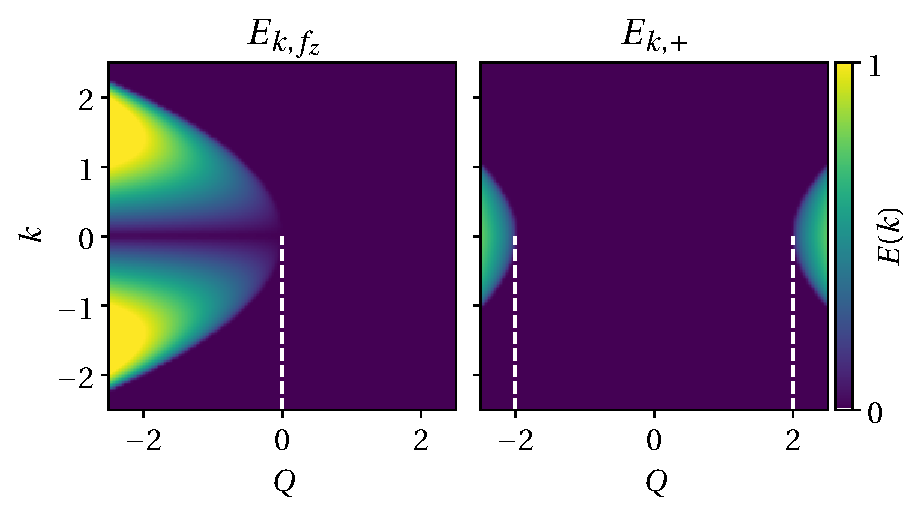
\includegraphics[width=0.75\textwidth]{gfx/ch-spin1/bogoliubov_energies.pdf}
    \caption[Real and imaginary parts of the Bogoliubov energies for the
        broken-axisymmetry phase of a spin-1 BEC]
    {Imaginary parts of the energies defined in Eq.~\eqref{eq: e_k-fz} and
    Eq.~\eqref{eq: e_k-pm} in a parameter space of mode \(k\) and
    \( Q=q/|c_1|n \).\label{fig: dens-spin-energies}}
\end{figure}
For \(|Q|>2\), \(\text{Im}(E_{k, +})\) becomes non-zero, indicating an
instability.
The critical point \(Q = 2\) corresponds to the second-order phase transition
from the polar to the BA phase, indicating that \(E_{k, +}\) is the desired
Bogoliubov energy for that particular transition.
However, we see that for \(Q<0\) the imaginary part of \(E_{k, f_z}\) becomes
non-zero, and hence unstable.
This critical point corresponds to the transition between the BA and FM phases,
which precisely describes our transition of interest.
Therefore, \(E_{k, f_z}\) is the correct Bogoliubov mode for our transition.
Note that for \(k=0\) an instability does not occur in the \(E_{k, f_z}\) mode,
and so studies focussing on this mode in particular will not capture the phase
transition that occurs at \(Q=0\)~\cite{Matuszewski2009, Qiu2020,
Mirkhalaf2021}.
In contrast, choosing the \(k=0\) mode is sufficient to capture the phase
transition at \(Q=2\) since it is the most unstable mode indicated in
\(E_{k, +}\).
In practice, the \(Q=-2\) transition is not realised since the instability at
\(Q=0\) for any \(k \neq 0\) will typically arise and take precedent when
\(Q\) is quenched from positive to negative values.

With the relevant Bogoliubov mode found, we can predict the scaling of the
density of defects for a BA to FM phase transition.
Since our relevant mode is gapless, it is instructive to consider a special case
of the spectrum, given as
\begin{align}\label{eq: dispersion-relation}
    \omega^2 \sim |q-q_c|^{\theta^+}k^{z^+}+k^{2z}.
\end{align}
We focus on the (+) spectrum (i.e., approaching the critical point from the BA
phase), since this determines the crossover from the adiabatic regime to the
impulse regime which sets the metastable state after the QDCP is crossed.
To be consistent with the KZM, where \(\omega \sim |q(t)-q_c|^{z}\), we make
the ansatz \(k \sim \xi^{-1} \sim |q(t)-q_c|^{\nu}\).
For a scaling solution to arise that is consistent with the relaxation time,
we require \(\omega sim k^z\).
This, combined with Eq.~\eqref{eq: dispersion-relation}, leads us to the
relation
\begin{align}
    \theta^+ = \nu (2z-z^+).
\end{align}
Now, in our system, we have \(q_c = 0\) and \(q = -t/\tau_Q\) and thus
Eq.~\eqref{eq: dispersion-relation} simplifies to
\begin{align}
    \omega^2 \sim \frac{|t|^{\theta^+}}{\tau_Q^{\theta^+}}k^{z^+}.    
\end{align}

Recall now the adiabatic-impulse approximation described in
Sec.~\ref{sec: the-KZM}, with an energy gap given by \(\Delta(t)\).
In this case, the relaxation time scales as \(\tau \sim 1/\Delta \), which
implies that far from the critical point the relaxation time is small, and the
system adiabatically follows the instantaneous ground state.
However, as the critical point is approached, \(\Delta \rightarrow 0\), and the
relaxation time then diverges.
At some time \(\tilde{t}\) the reaction time becomes comparable to the
transition time, \(\Delta / \dot{\Delta}\), and the system can no longer
adiabatically follow the ground state.
This time (often denoted the freezing time), \(\tilde{t}\), denotes the onset
of the impulse regime, where the system becomes frozen.
Therefore, the freezing time can be evaluated from the expression
\begin{align}
    \frac{1}{\Delta(\tilde{t})} \sim
    \frac{\Delta(\tilde{t})}{\dot{\Delta}(\tilde{t})} .
\end{align}

\section{Numerical studies of the KZM across a first-order phase transition}
\subsection{Broken-axisymmetry to ferromagnetic quench}
The KZM typically concerns second-order phase transitions. However, recent
work has been conducted in condensed matter systems which investigate
the KZM across first-order transitions~\cite{Qiu2020}.
We aim to extend this research and present results for
the first-order transition between the broken-axisymmetry and
ferromagnetic phases.

We start from the broken-axisymmetry (BA) wave function with \( p=0 \)
\begin{equation}
    \psi_{\pm 1} = \frac{\sqrt{2}}{4}\sqrt{2 - Q(t)}, \qquad
    \psi_0 = \frac{1}{2}\sqrt{2 + Q(t)},
    \label{eq: BA-initial-wavefunction}
\end{equation}
where \(Q(t)=q(t)/|c_1|n\).
The BA wave function is the ground state for \(c_1 < 0\) and \(0 < Q < 2\).
There exists a critical point at \( Q = 0 \) where the ground state changes from
the BA phase to the ferromagnetic phase.
We perform 1D simulations on a grid of \(N_x = 16384\) grid points with a grid
spacing of \(\Delta_x = 0.125\).
We perturb the initial BA state by adding small noise, \(\delta_m\), to each
component where \(|\delta_m| \ll 1\), and we generate the real and imaginary
parts of \(\delta_m\) for each grid point using the probability distribution
\(p(x) = e^{-x^2/2\sigma^2}{(\sqrt{2\pi}\sigma)}^{-1}\) where we choose
\(\sigma=10^{-4}\) so that we start close to the BA ground state.

\subsection{Phase boundaries in the ferromagnetic phase}
As the system is quenched across the critical point at \( Q = 0 \), the ground
state changes to the ferromagnetic phase.
The order parameter for this phase takes the form \(\zeta={(1,0,0)}^T\) or
\(\zeta={(0,0,1)}^T\) depending on the orientation of the spin.
From Eq.~\eqref{eq: BA-initial-wavefunction} we have
\(\psi_{\pm 1} = \frac{1}{2}\) and \(\psi_0 = \frac{\sqrt{2}}{2}\) at
\( Q = 0 \).
The question that remains is: Which state will the system choose after
the critical point is passed?

\begin{figure}[tb]
    \centering
    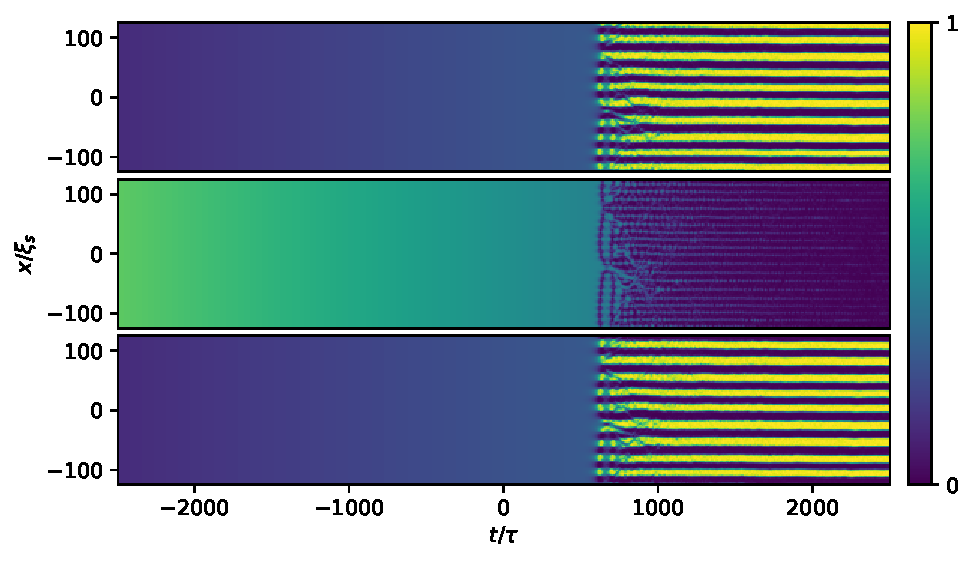
\includegraphics[width=\textwidth]{gfx/ch-spin1/BA-FM_all_densities.pdf}
    \caption[Component densities of the system as a function of time]
    {Plots of \(|\psi_1|^2\) (top) \(|\psi_0|^2\) (middle) and
        \(|\psi_{-1}|^2\) (bottom) as a function of time for a \(256\xi_s\)
        spatial subregion of the condensate for
        \( \tau_Q=2500\tau \).\label{fig: BA-FM-densities}}
\end{figure}
Fig.~\ref{fig: BA-FM-densities} shows the full evolution of the density of each
component for a quench time \( \tau_Q=5000\tau \).
As the Zeeman shift is quenched, we see the density of the \(\psi_0\) component
linearly decrease as the \(\psi_{\pm 1}\) components increase.
After the critical point at \(t/\tau=0\) is passed there is a freeze-out time
(see Sec.~\ref{sec: the-KZM}) before the system crosses into the ferromagnetic
phase.
During this new phase, we see the formation of ferromagnetic domain walls
(characterised by the bright density peaks) in the \(\psi_{\pm 1}\) components
as the order parameter adjusts to the new ground state.
These domains are spatially separated and where there is zero density in one of
the components, there is maximal density in the other so that overall the total
density \(n=\sum_m\psi_m^*\psi_m\) is uniform.

The KZM predicts in Eq.~\eqref{eq: KZM-domain-size} that the size of the domains
grow as the quench time increases.
\begin{figure}[tb]
    \centering
    \begin{subfigure}{0.45\textwidth}
        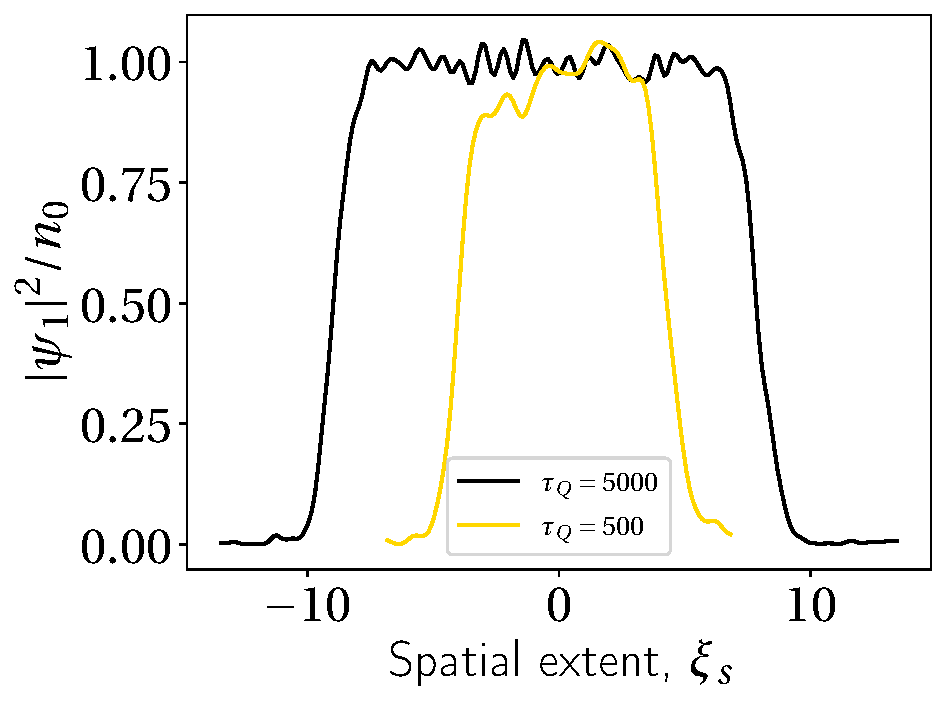
\includegraphics[width=\textwidth]{gfx/ch-spin1/BA-FM_domain_width.pdf}
        \caption{\label{fig: BA-FM-domain-width-comparison}}
    \end{subfigure}
    \begin{subfigure}{0.45\textwidth}
        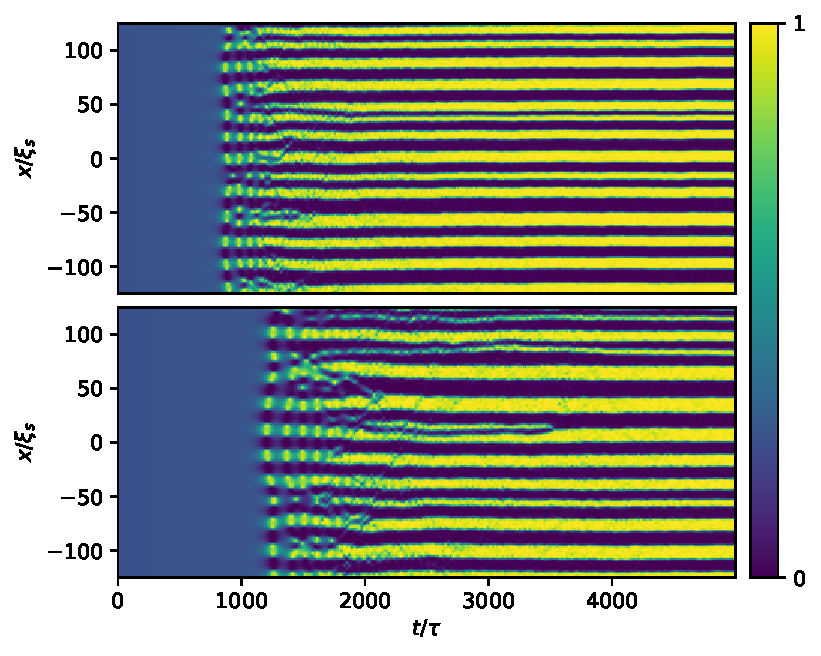
\includegraphics[width=\textwidth]{gfx/ch-spin1/BA-FM_domain_onset.pdf}
        \caption{\label{fig: BA-FM-domain-onset}}
    \end{subfigure}
    \caption[Density profile across an average FM domain]
    {(a): Density profile of the \(\psi_1\) component across an average
        domain in a simulation with \(\tau_Q=2500\tau \) (black line) and
        \(\tau_q=10000\) (red line).
        (b): Time evolution of \( |\psi_1|^2\) for a \(256\xi_s\) spatial subregion
        for \( \tau_Q=5000\tau \) (top) and \(\tau_Q=10000\tau \) (bottom).}
\end{figure}
Fig.~\ref{fig: BA-FM-domain-width-comparison} shows the average domain size
for two different simulations with \(\tau_Q=2500\) and \(\tau_Q=10000\).
We see that the longer quench time produces domains that have a
larger width than those of faster quenches, supporting the Kibble-Zurek theory.
In addition, we plot the time evolution of \(|\psi_1|^2\) for \(\tau_Q=5000\) and
\(\tau_Q=10000\) in Fig.~\ref{fig: BA-FM-domain-onset}.
We see the ferromagnetic domain formation is delayed in the simulation
with a longer quench time, which supports the prediction in
Eq.~\eqref{eq: freeze-out-scaling}.

One can count the number of ferromagnetic domains in the system and see the
dependence on \( \tau_Q \).
To do this, we developed a numerical algorithm that counts the number of
density peaks in each component and sums the result to give the total number of
domains, \(N_d\).
We calculate this quantity at time \(t/\tau=\tau_Q/2\) in each simulation, to
ensure that the domains are frozen and avoid the early-time coarsening
taking place which could affect the total number of domains present.
\begin{figure}
    \centering
    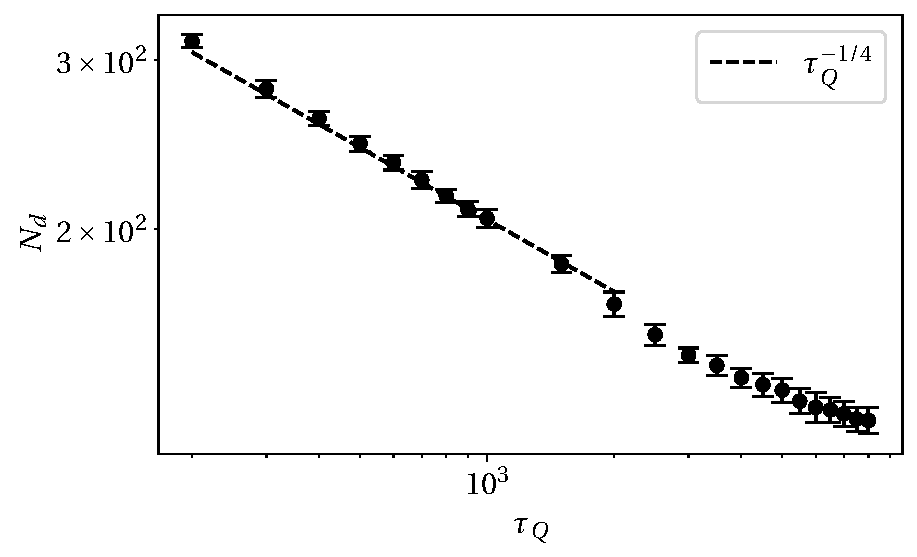
\includegraphics[width=0.65\textwidth]{gfx/ch-spin1/FM_domains_scaling.pdf}
    \caption[Total ferromagnetic domains in the system versus the quench rate
        \(\tau_Q\)]
    {The number of ferromagnetic domains as a function of the
        quench time. Each point represents 50 simulations and the
        error bar gives one standard deviation. Overlaid are the scaling lines
        \(\tau_Q^{-1/3}\) (black dashed line) and \(\tau_Q^{-1/5}\)
        (red dotted line).\label{fig: FM-domains-scaling}}
\end{figure}
In Fig.~\ref{fig: FM-domains-scaling} we plot the total number of domains
as a function of the quench time with fifty ensemble runs for each simulation.
We see that there is not a uniform scaling throughout all quench times tested.
Faster quenches indicate a steeper power-law scaling of the number of domains
that approaches \(N_d\sim\tau_Q^{-1/3}\).
As the quench time slows, a deviation from this scaling takes place at
approximately \(\tau_Q\approx 3\times10^3\tau \), where the scaling of the
domains approaches \(N_d\sim\tau_Q^{-1/5}\).
\textcolor{red}{I guess the question now is: why is there a deviation?
    Is the larger domain size (due to slower quench times) affecting the scaling?
    Is it a consequence of the grid size? Can the \(1/3\) scaling be linked to KZ
    theory?}

\subsection{Power-law scaling near the critical point}
Since we know the relevant unstable mode within our system, we can investigate
power-law scaling near the critical point.
To begin, we start with the fluctuation operator associated with the
Bogoliubov spectrum \(E_{\vb{k}, fz}\)
\begin{equation}
    \hat{a}_{\vb{k}, {f_z}} = \frac{1}{\sqrt{2}}(\hat{a}_{\vb{k}, 1}
    - \hat{a}_{\vb{k}, -1}),
    \label{eq: fz-fluctuation-operator}
\end{equation}
where \(\hat{a}_{\vb{k}, \pm1}\) is the annihilation operator for a spin-1 boson
with wave number \( \vb{k} \) in component \(m=\pm1\).
\begin{figure}[tb]
    \centering
    \begin{subfigure}{0.45\textwidth}
        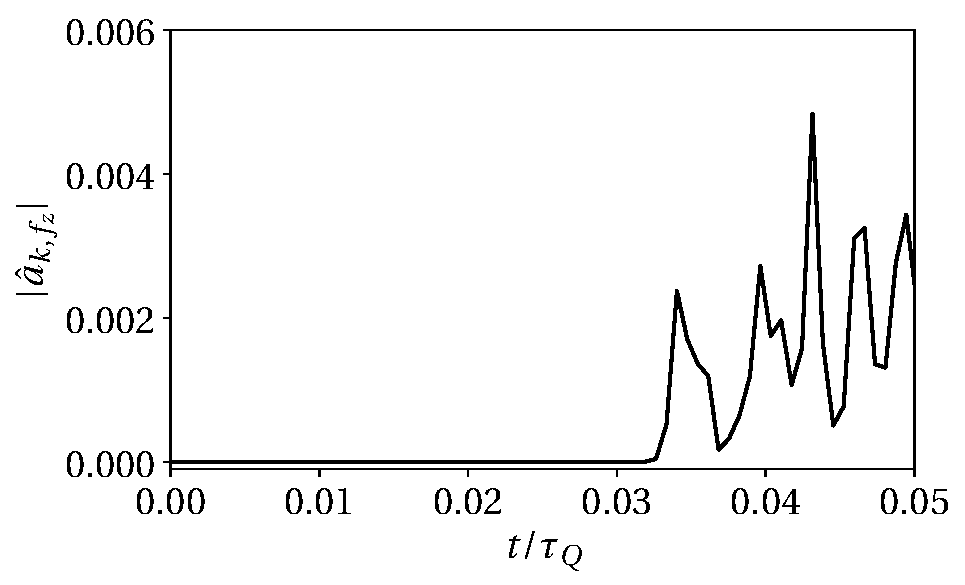
\includegraphics[width=\textwidth]
        {gfx/ch-spin1/1d_BA-FM_5000_fluctuation_diff.pdf}
        \caption{\label{fig: fluctuation-diff}}
    \end{subfigure}
    \begin{subfigure}{0.45\textwidth}
        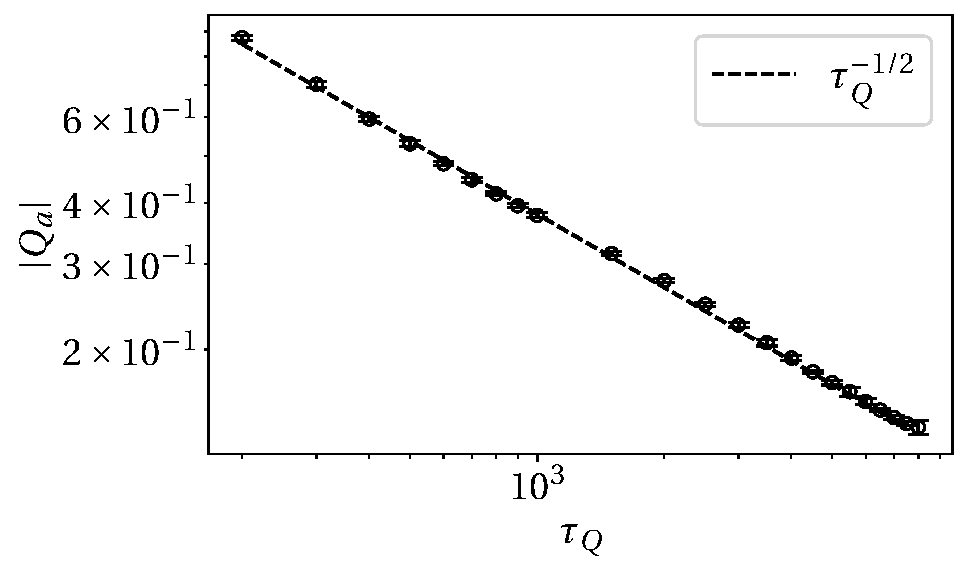
\includegraphics[width=\textwidth]{gfx/ch-spin1/BA-FM_Qa_scaling.pdf}
        \caption{\label{fig: Q_a-scaling}}
    \end{subfigure}
    \caption[Growth of the fluctuation operator]
    {(a): The modulus of the fluctuation operator in
        Eq.~\eqref{eq: fz-fluctuation-operator} for \(\vb{k}=1\) and
        \(\tau_Q=5000\).
        The plot shown is obtained by averaging over all runs in the ensemble.
        (b): The critical value \(Q_a\) as a function of the quench time.
    }
\end{figure}
Fig.~\ref{fig: fluctuation-diff} shows the above quantity for a quench time
of \(\tau_Q=5000\) with \(\vb{k}=1\).
The quantity remains zero until after the critical point is passed, where
a rapid period of growth occurs.
This onset of this growth corresponds to the ferromagnetic domains forming
within the system (see Fig.~\ref{fig: BA-FM-densities}).
Motivated by previous work~\cite{Damski2007, Qiu2020}, we define a time,
\( \hat{t} \), which is the time when \(|\hat{a}_{\vb{k}, {f_z}}|\) first
exceeds 1\% of its maximum value: \(|\hat{a}_{\vb{k}, {f_z}}(\hat{t})| =
0.01\times \max|\hat{a}_{\vb{k}, {f_z}}(t)|\).
For the system in Fig.~\ref{fig: fluctuation-diff}, we obtain
\(\hat{t}=598\tau \).
Using this time, we can extract the critical value of \( q \) that this growth
occurs at, \(Q(\hat{t}) = Q_a\).
Fig.~\ref{fig: Q_a-scaling} shows \(Q_a\) as a function of the quench time.
We see a clear power-law scaling of \(Q_a \propto \tau_Q^{-\frac{1}{2}}\) for
all values of \( \tau_Q \) tested.
This exponent differs from observed results in previous works investigating
second-order phase transitions~\cite{Damski2007, Anquez2016, Swislocki2013}
where an exponent of \(-1/3\) is observed.
Our observation of a \(-1/2\) exponent signifies a deviation from
the Kibble-Zurek theory which appears to be a consequence of our transition
being first-order.

\subsection{Extracting a power-law scaling near the critical point}
Having identified the relevant mode of the transition, we now follow a procedure
similar to Damski~\cite{Damski2007} and analytically determine the scaling
behaviour of the system near the critical point.

To begin, we start with a wave function close to the BA state
\begin{equation}\label{eq: spin-1-perturbed-BA-state}
    \Psi^T = \left(\frac{\sqrt{2n_0}}{4}\sqrt{2 - Q_0} + \delta\psi_{1}(t),
    \frac{\sqrt{n_0}}{2}\sqrt{2 + Q_0} + \delta \psi_0(t),
    \frac{\sqrt{2n_0}}{4}\sqrt{2 - Q_0} + \delta\psi_{-1}(t)\right)e^{-i\mu t},
\end{equation}
where \( 0 < Q_0 < 2 \) is a constant, \(\mu \) is the
chemical potential and \( |\delta\psi_m| \ll 1 \) are time-dependent noise
terms.
The noise terms must satisfy \(\int \sum_m\delta\psi_m+\delta\psi_m^* \, \dd z\)
to ensure normalisation of the wave function.
Additionally, they must also satisfy \(\int (\delta\psi_1 + \delta\psi_1^* 
\delta\psi_{-1} + \delta\psi_{-1}^*) \dd z = 0\) to ensure that magnetisation
is conserved.

Recall the spin-1 GPEs are given as (see Sec.~\ref{subsec: spin-1-gpes}):
\begin{align}\label{eq: spin-1-KZ-GPEs}
    i\hbar\pdv{\Psi}{t} = \left[ -\frac{\hbar^2\nabla^2}{2M}
    -p\hat{F_z} + q\hat{F}_z^2 +c_0n +c_1n\langle \hat{\vb{F}}\rangle
    \cdot \hat{\vb{F}}\right]\Psi.
\end{align}
Substituting Eq.~\eqref{eq: spin-1-perturbed-BA-state} into the above equations
and keeping leading order terms in \(\delta\psi_m\) yields the following two
equations for \(\delta_{\pm 1}\) (\(p=0\))
\begin{multline}\label{eq: dpsi1}
    i\hbar\pdv{\delta\psi_1}{t} = \left[-\frac{\hbar^2}{2M}\dv[2]{}{z}+q-\mu
    + \frac{n_0(10c_0+6c_1-(c_0-c_1)Q)}{8}\right]\delta\psi_1 \\
    + \frac{n_0\sqrt{2(4-Q^2)}}{8}\left[
        (c_0 + 3c_1)\delta\psi_0
        + (c_0+c_1)\delta\psi_0^*
    \right] \\
    + \frac{n_0(2-Q)}{8}\left[(c_0-c_1)\delta\psi_{-1}
    + (c_0+c_1)\delta\psi_1^*\right]
    + \frac{n_0}{8}\left[(2-Q)c_0 + (2+3Q)c_1\right]\delta\psi_{-1}^*,
\end{multline}
\begin{multline}\label{eq: dpsim1}
    i\hbar\pdv{\delta\psi_{-1}}{t} = \left[-\frac{\hbar^2}{2M}\dv[2]{}{z}+q-\mu
    + \frac{n_0(10c_0+6c_1-(c_0-c_1)Q)}{8}\right]\delta\psi_{-1} \\
    + \frac{n_0\sqrt{2(4-Q^2)}}{8}\left[
        (c_0 + 3c_1)\delta\psi_0
        + (c_0+c_1)\delta\psi_0^*
    \right] \\
    + \frac{n_0(2-Q)}{8}\left[(c_0-c_1)\delta\psi_{1}
    + (c_0+c_1)\delta\psi_{-1}^*\right]
    + \frac{n_0}{8}\left[(2-Q)c_0 + (2+3Q)c_1\right]\delta\psi_{1}^*.
\end{multline}
Now, subtracting Eq.~\eqref{eq: dpsim1} from Eq.~\eqref{eq: dpsi1} results in
the following ordinary differential equation
\begin{align}\label{eq: G_y-unsimplified}
    i\hbar\dv{G_y}{t}= \left[ -\frac{\hbar^2}{2M}\dv[2]{}{z}+q
    -\mu+n_0(c_0+c_1)\right]G_y
    -\frac{c_1n_0Q}{2}G_y^*,
\end{align}
where \(G_y = \delta\psi_1 - \delta\psi_{-1}\).
The chemical potential of the system is calculated from the \(\psi_0\)
component of Eq.~\eqref{eq: spin-1-KZ-GPEs}, again keeping leading order terms
in \(\delta\psi_0\) and assuming a stationary state, leading to
\(\mu=c_0n_0 + c_1n_0(2 - Q_0)/2\).
Using this expression for the chemical potential and \(q(t) = -c_1n_0Q(t)\)
Eq.~\eqref{eq: G_y-unsimplified} simplifies to
\begin{align}\label{eq: G_y-simplified}
    i\hbar\dv{G_y}{t} = \left[ -\frac{\hbar^2}{2M}\dv[2]{}{z}
    -c_1n_0\left(Q-\frac{Q_0}{2}\right)\right]G_y
    - \frac{c_1n_0Q}{2}G_y^*.
\end{align}

We now split \(G_y\) into real and imaginary parts and make use of Fourier
transforms, \(a_y=\int \text{Re}(G_y)e^{ikz} dz\) and
\(b_y=\int \text{Im}(G_y)e^{ikz} dz\) to progress our analysis.
Substituting these expressions in Eq.~\eqref{eq: G_y-simplified} yields the
following matrix equation
\begin{align}\label{eq: a_y-matrix}
    \dv{t}\mqty[a_y \\ b_y] = \mqty(0 & \frac{\hbar k^2}{2M}
    - \frac{c_1  n_0}{2\hbar}(Q - Q_0) \\
    \frac{c_1  n_0}{2\hbar} \left( 3Q-Q_0 \right)-\frac{\hbar k^2}{2M} & 0)
    \mqty[a_y \\ b_y].
 \end{align}
To solve the above matrix equation, we construct the equation for
\(\dv[2]{a_y}{t}\) and substitute the critical point value \(Q=0\) to obtain
\begin{align}
    \dv[2]{a_y}{t} = \frac{c_1n_0}{2\hbar\tau_Q}b_y
    + \left(\frac{\hbar^2k^2}{2M} - \frac{c_1n_0Q}{2\hbar}\right)\dv{b_y}{t}.
\end{align}
Now, expressions for \(b_y\) and \(\dv{b_y}{t}\) are found from
Eq.~\eqref{eq: a_y-matrix}, which transforms the above equation to
\begin{align}
    \dv[2]{a_y}{t} = \frac{1}{\tau_Q\left(\frac{\hbar^2k^2}{Mc_1n_0}
    - Q\right)}\dv{a_y}{t}
    - \left(\frac{\hbar^2k^4}{4M^2} - \frac{k^2c_1n_0Q}{M}
    + \frac{3c_1^2n_0^2Q^2}{4\hbar^2}\right)a_y.
\end{align}
Finally, to simplify the above expression, we use the spin healing length
\(\xi_s = \hbar/\sqrt{2|c_1|n_0}\) and the spin time \(\tau_s=\hbar/|c_1|n_0\):
\begin{align}
  \dv[2]{a_y}{t} = \frac{-1}{\left(2\xi_s^2 k^2 \tau_Q- t \right)}\dv{a_y}{t}
  -\left( \frac{\xi_s^4 k^4}{4\tau_s^2} -\frac{\xi_s^2 k^2 t}{2\tau_s^2 \tau_Q}
  + \frac{3 t^2}{16\tau_s^2 \tau_Q^2} \right) a_y.
\end{align}

Now, to extract scaling solutions, we rescale time as \(t rightarrow t\lambda \)
where \(\lambda = \sqrt{\tau_s\tau_Q}\), which leads to the final differential
equation
\begin{align} \label{eq: eqn-scaled-lin}
    \dv[2]{a_y}{t} = \frac{-1}{\left( 2\kappa^2 - t\right)}\dv{a_y}{t}
    -\frac{1}{4} \left( \kappa^4 - 2\kappa^2 t + \frac{3 t^2}{4} \right)a_y,
\end{align}
where \(\kappa^2 = \xi_s^2 k^2 \sqrt{\tau_Q/\tau_s}\).
This scaling ensures that the last term of the above equation is independent of
\(\tau_Q\).
Then, the remaining dependence on \(\tau_Q\) is eliminated if we require that
\(\kappa \) is constant, implying that \(\kappa \sim \tau_Q^{-1/4}\).
Under these conditions, we expect scaling solutions to arise which are then
consistent with the derived scaling for both the correlation length and
dynamical exponents based on the KZM\@.

\subsection{Crossing two phase transitions}
To test the robustness of the observed scaling, we combine the effort of the
previous two numerical studies into one.
Namely, we investigate the scaling of the density of defects using a simulation
that spans two phase transitions.
Starting from the polar phase at \(Q  = 2.5\), we quench the quadratic Zeeman
shift such that we cross over to the BA phase at \(Q=2\) and finally the FM
phase at \(Q=0\).
This quench then evidently spans two phase transitions: one second-order, and
one-first order.
Our numerical set up is exactly the same as the previous section.

\begin{figure}
    \centering
    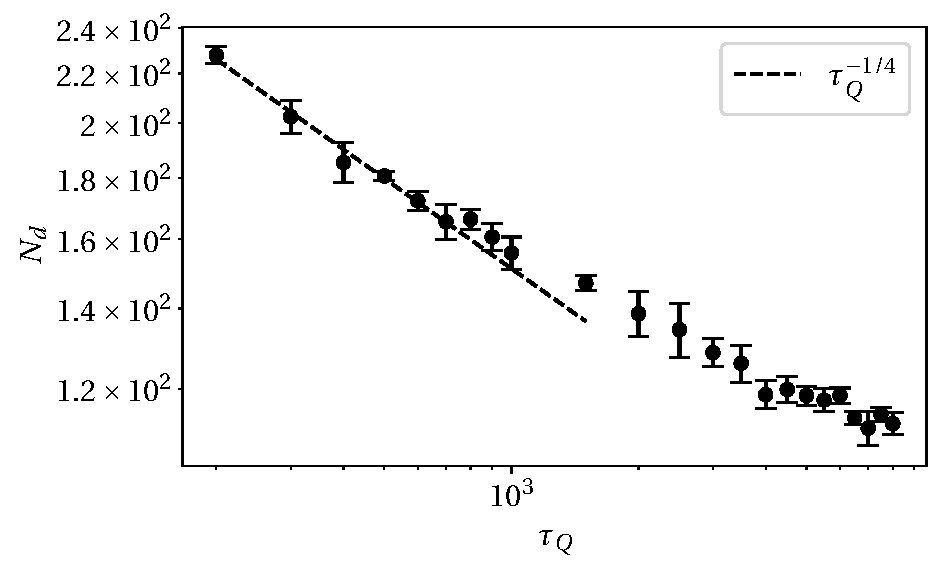
\includegraphics[width=0.75\textwidth]{gfx/ch-spin1/polar-BA-FM_domains.pdf}
    \caption{\label{fig: polar-ba-fm-defects}Number of ferromagnetic domains as
    a function of the quench time, \(\tau_Q\), after the system has crossed two
    phase transitions.
    Each point is averaged over 5 runs, with the error bars giving \(\pm 1\)
    standard deviation.}
\end{figure}
We once again count the number of ferromagnetic domains present at the end of
the simulation when the system is in the FM phase.
Results for the density of defects are plotted in
Fig.~\ref{fig: polar-ba-fm-defects}.
Despite passing through two phase transitions, we observe qualitatively similar
behaviour to that of previous transition crossing only the first-order phase
transition (see Fig.~\ref{fig: FM-domains-scaling}).
For fast quenches (\(\tau_Q \lesssim 10^3 \)), the scaling of the density of
defects follows closely to \(N_d \sim \tau_Q^{-1/4}\).
Similar to the previous case, there is a deviation from this scaling when the
quench time becomes slower (\(\tau_Q > 10^3\)).
This shows that the scaling of the density of defects for fast quenches is
robust, and is unaffected by the number of previous phase transitions.